\section{Introduction}
\textcolor{red}{Because of lack of a better place I will make a metacomment here regarding general structure. I think the general structure should be the following: 1. Introduction 2. Context 3. Related work 4. Methodology 5. Results and Discussion 5. Conclusion.
\begin{enumerate}
    \item 1. Introduction: add extension that includes summary and contributions. <2 pages max>
    \item Move 2.1, 2.2, 2.3 2.4 here. Should be the chapter that informs reader about DNNs, phonemes etc. <5-7 pages>
    \item  Related Work: focus on the main point which is compensation (lexical ), Bursic and Busso etc. What is your state-of-the-art you compare against and other methods. Should be short but comprehensive. <2-3 pages>
    \item  Have subsection here with models, datasets, etc. Sec 3 should be here, 4 as well, 5 as well 2.5 , 2.6. 
    \item  Organise along important questions you are researching. Include results and discussion for every question.
    \item  Conclusion <2-3 pages>
\end{enumerate}
I am not sure of the right balance between 4 and 5. A (maybe better) alternative would be to have a single 4+5 section and for each research question you comment methodology, results and discussion.
}

The study of detecting and quantifying human emotion has been a topic for many years. Going back to 1894, William James proclaimed that emotion is a result of our actions \cite{james1948emotion}. More important though was his idea that emotion correlates to feeling \cite{james2007principles}. Emotions themselves are induced by stimuli, which excite the human subject and thus propagates to bodily change. According to Izard, the core theories that view cognitive and sensory processes as emotional activators can be followed back to James \cite{izard1990substrates}.

Going forward several years into the mid-90s, Picard consolidated ideas of computing and measuring affect in her 1995 essay, coining the term Affective Computing \cite{picard2000affective}. A subfield of affective computing is based around recognising affective states from facial expressions. Much of the progress in this field bases its research around several axiomatic assumptions, one of which being that all facial movements are induced by emotion. This is especially problematic if the analysed subject is speaking, since the act of talking also triggers facial movement and thus introduces noise into the input data. 

In this thesis, we want to find ways to make existing facial expression recognition models more robust towards talking subjects.

\textcolor{red}{This can be its own subsection, entitled for example "Summary and Contributions".}

\textcolor{red}{We explore two main approaches for increasing robustness: 
\begin{enumerate}
    \item Temporal compensation.
    \item Lexical compensation.
\end{enumerate} 
In the case of temporal compensation we do a), b) c) state here the main things done like we adopt state-of-the-art recurrent DNNs that are able to capture temporal information. ...
in the case of lexical compensation we do a) lexical compensation 1. The core idea is to ... <core idea of bursic> b) lexical compensation 2 ... <core idea of busso> etc.
We proceed with a comprehensive analysis of robustness. Mainly we were interested in answering the following questions: 
\begin{enumerate}
    \item How does compensation compare to human recognition? For answering this we: 
    \begin{enumerate}
        \item Performed data collection etc. etc. 
        \item Implemented labelling toll etc. 
    \end{enumerate}
    Main results showed that ...
    \item Is compensation robust to domain shift?
    We performed an analysis of domain shift evaluation by testing our models on additional datasets etc. etc.
    Main result showed that ...
    \item Is compensation language agnostic?
    We did that and that ...
    Results showed that ...
    \item ...?
\end{enumerate}
}

We will analyse how humans detect emotion when confronted with speaking people (Chapter \ref{sec:human}), and try to include those findings in our models (Chapter \ref{sec:models}). We further benchmark our models against inputs of different languages, and speech acts that are more akin to those in the real world (Chapter \ref{sec:data}).

We conclude our work with an analysis of the different modalities of our models, and give an outlook into further research towards a more robust framework of facial emotion recognition that contextualises speech.

\begin{figure}
    \centering
    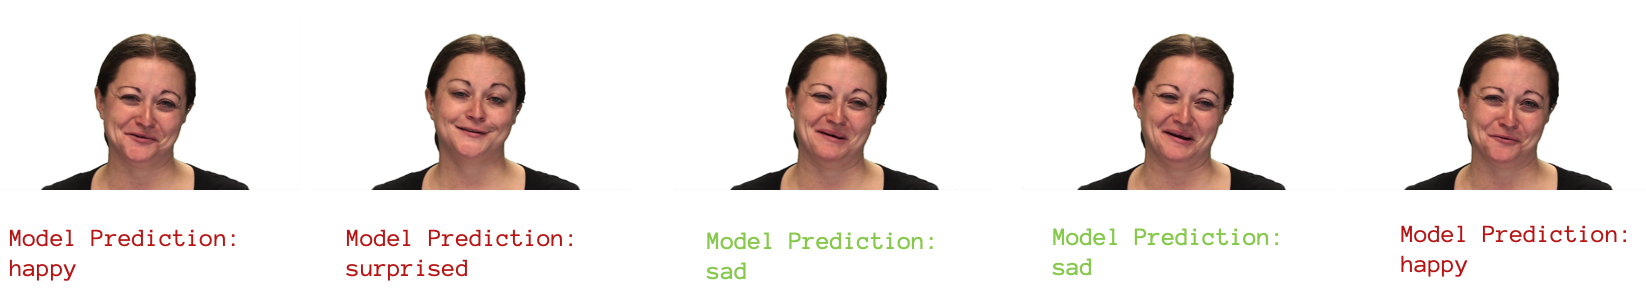
\includegraphics[width=0.8\textwidth]{res/modelex.png}
    \caption{An example of a model mislabeling a speaking subject talking while expressing a \texttt{sad} emotion \cite{livingstone2018ryerson}. Ideally, all frames, or the collection of frames, would be correctly categorized as \texttt{sad}.}
    \label{fig:mislabel}
\end{figure}